\documentclass[tikz,border=12pt]{standalone}
\usepackage[T1]{fontenc}
\usepackage{tgheros}
\usepackage{sfmath}
\usepackage{amsmath}
\usepackage{amssymb}
\usepackage{fontawesome5}
\usepackage{tikz}
\usetikzlibrary{arrows.meta,positioning,shapes.geometric,fit,backgrounds,calc}
\usepackage{xcolor}

\renewcommand{\familydefault}{\sfdefault}

% Harvard Crimson & ETH Zurich Academic Semantic Palette
\definecolor{harvardcrimson}{HTML}{A51C30}
\definecolor{ethdarkblue}{HTML}{1F407A}
\definecolor{ethblue}{HTML}{215CAF}
\definecolor{ethpetrol}{HTML}{007A87}
\definecolor{ethbronze}{HTML}{B87333}
\definecolor{ethpurple}{HTML}{5B4B8A}
\definecolor{ethslate}{HTML}{475569}
\definecolor{cardbg}{HTML}{F8FAFC}
\definecolor{cardborder}{HTML}{CBD5E1}
\definecolor{safeTeal}{HTML}{10B981}
\definecolor{alertRed}{HTML}{DC2626}

\begin{document}
\begin{tikzpicture}[
  font=\sffamily,
  >=Stealth,
  flowbox/.style={
    draw=cardborder,
    fill=cardbg,
    rounded corners=4pt,
    line width=0.8pt,
    minimum height=1.30in,
    inner sep=6pt,
    align=center,
    anchor=north
  }
]

  % Top Title Banner
  \node[draw=ethdarkblue, fill=ethdarkblue!5, rounded corners=5pt, line width=1pt, text width=9.20in, inner sep=7pt, align=center] (title) at (4.60in, 0) {
    {\normalsize\bfseries\color{ethdarkblue}\faIcon{cube}\;\; SPATIAL AFFORDANCE TOKENIZATION VS. PASSIVE CLASSIFICATION}\\[2pt]
    {\scriptsize\color{ethslate}Lifting 2D Pixels into 3D Metric Affordance Tokens for Action Decoders and World Models}
  };

  % Input: RGB-D Image
  \node[flowbox, draw=ethblue!70, text width=1.55in] (input) at (0.80in, -0.65in) {
    {\scriptsize\bfseries\color{ethblue}\faIcon{camera}\; RAW OBSERVATION}\\[3pt]
    {\scriptsize\bfseries RGB-D Stream}\\[4pt]
    {\tiny\color{ethslate}Calibrated RGB + Depth\\[2pt]$640 \times 480 \times 4$\\[2pt]DMA Coherent Buffer}\\[6pt]
    \rule{0.85\linewidth}{0.3pt}\\[4pt]
    {\scriptsize\textbf{\color{ethblue}$I_t \in \mathbb{R}^{H \times W \times 4}$}}
  };

  % Patch Tokenization & Vision Backbone
  \node[flowbox, draw=ethpetrol!80, text width=1.70in] (vit) at (2.95in, -0.65in) {
    {\scriptsize\bfseries\color{ethpetrol}\faIcon{th-large}\; SPATIAL ENCODER}\\[3pt]
    {\scriptsize\bfseries ViT / DINOv2 Backbone}\\[4pt]
    {\tiny\color{ethslate}$14 \times 14$ Patch Extraction\\[2pt]Multi-Head Self-Attention\\[2pt]Dense Feature Extraction}\\[6pt]
    \rule{0.85\linewidth}{0.3pt}\\[4pt]
    {\scriptsize\textbf{\color{ethpetrol}$z_{\text{vis}} \in \mathbb{R}^{N \times D_{\text{model}}}$}}
  };

  % Divergence into Two Approaches
  % Top Branch: Passive Classification
  \node[flowbox, draw=alertRed!70, fill=alertRed!5, text width=3.80in, minimum height=1.15in] (passive) at (6.70in, -0.65in) {
    {\scriptsize\bfseries\color{alertRed}\faIcon{times-circle}\; PASSIVE CLASSIFICATION (Digital ML Paradigm)}\\[3pt]
    {\tiny\color{ethslate}
    $\bullet$ Global Average Pooling over spatial patch grid\\
    $\bullet$ Emits categorical probability vector: $p(\text{"ceramic mug"}) = 0.94$\\
    $\bullet$ \textbf{Physical AI Failure:} Contains zero metric coordinates, zero contact normals, zero grasp reachability, and zero collision boundaries. Unusable by motor controllers.
    }
  };

  % Bottom Branch: Spatial Affordance Tokens
  \node[flowbox, draw=safeTeal!80, fill=safeTeal!5, text width=3.80in, minimum height=1.50in] (affordance) at (6.70in, -2.15in) {
    {\scriptsize\bfseries\color{safeTeal}\faIcon{check-circle}\; 3D SPATIAL AFFORDANCE TOKENS (Physical AI Paradigm)}\\[3pt]
    {\tiny\color{ethslate}
    $\bullet$ \textbf{3D Metric Unprojection:} $\mathbf{P}_{3D} = \mathbf{T}_{C}^{W} \cdot \mathbf{K}^{-1} [u, v, 1]^T \cdot d(u,v)$\\
    $\bullet$ \textbf{Metric Grasp Frame:} $\mathbf{T}_{\text{grasp}} = [\mathbf{p}_{\text{target}}, \mathbf{q}_{\text{quat}}] \in SE(3)$\\
    $\bullet$ \textbf{Surface Normal \& Friction:} $\hat{\mathbf{n}} \in \mathbb{S}^2, \;\; \hat{\mu}_{\text{friction}} = 0.45 \pm 0.05$\\
    $\bullet$ \textbf{Obstacle Clearance Boundary:} $r_{\text{clearance}} = 0.08\text{ m}$ (for CBF Invariant)
    }
  };

  % Connecting Arrows
  \draw[->, line width=1.1pt, draw=ethdarkblue] (input.east) -- (vit.west);
  \draw[->, line width=1.1pt, draw=alertRed] (vit.east) -- ++(0.35in, 0) |- (passive.west);
  \draw[->, line width=1.4pt, draw=safeTeal] (vit.east) -- ++(0.35in, 0) |- (affordance.west);

  % Bottom Output Destination Banner
  \node[draw=ethdarkblue, fill=ethdarkblue!10, rounded corners=4pt, line width=0.9pt, text width=9.20in, inner sep=5pt, align=center] (downstream) at (4.60in, -4.00in) {
    {\scriptsize\bfseries\color{ethdarkblue}\faIcon{arrow-right}\; DOWNSTREAM ACTION CONSUMPTION:}\;
    {\tiny\color{ethslate}Feeds directly into \textbf{Station 4} (Latent World Models), \textbf{Station 5} (1 Hz VLM Intent Leases), and \textbf{Station 6} (20 Hz Action Chunking Decoders)}
  };

  \draw[->, line width=1.1pt, draw=safeTeal] (affordance.south) -- (affordance.south |- downstream.north);

\end{tikzpicture}
\end{document}
